\documentclass[a4paper]{book}
\special{dvipdfmx:config z 0} %取消PDF压缩,加快速度,最终版本生成的时候最好把这句话注释掉

\usepackage{amssymb}
\usepackage{bookmark}
\usepackage[hypcap=false]{caption}
\usepackage{enumitem}	% 定制enumerate标号
\usepackage{geometry}
\geometry{
	left=2cm,
	right=2cm,
	top=2cm,
	bottom=2cm,
}
\usepackage{hyperref}
\hypersetup{
    colorlinks=true,            %链接颜色
    linkcolor=black,             %内部链接
    filecolor=magenta,          %本地文档
    urlcolor=cyan,              %网址链接
}
\usepackage[none]{hyphenat}		% 阻止长单词分在两行
\usepackage{mathrsfs}
\usepackage[version=4]{mhchem}
\usepackage{subcaption}
\usepackage{titlesec}

% setting about showing the contents
\setcounter{tocdepth}{3}
\setcounter{chapter}{5}

\RequirePackage[many]{tcolorbox}
\tcbset{
    boxed title style={colback=magenta},
	breakable,
	enhanced,
	sharp corners,
	attach boxed title to top left={yshift=-\tcboxedtitleheight,  yshifttext=-.75\baselineskip},
	boxed title style={boxsep=1pt,sharp corners},
    fonttitle=\bfseries\sffamily,
}

\definecolor{skyblue}{rgb}{0.54, 0.81, 0.94}

\newcounter{exercise}[chapter]
\newcounter{solution}[chapter]
\newcounter{eqs}[solution]

\newenvironment{sequation}
  {\begin{equation}\stepcounter{eqs}\tag{\thesolution-\theeqs}}
  {\end{equation}}

\newtcolorbox[use counter=exercise, number within=chapter, number format=\arabic]{exercise}[1][]{
    title={Exercise~\thetcbcounter},
    colframe=skyblue,
    colback=skyblue!12!white,
    boxed title style={colback=skyblue},
    overlay unbroken and first={
        \node[below right,font=\small,color=skyblue,text width=.8\linewidth]
        at (title.north east) {#1};
    }
    label={\unskip},
    before upper={
        \phantomsection
        \addcontentsline{toc}{subsubsection}{Exercise\hspace{1em}\thetcbcounter}
    },
}

\newtcolorbox[use counter=solution, number within=chapter, number format=\arabic]{solution}[1][]{
    title={Solution~\thetcbcounter},
    colframe=teal!60!green,
    colback=green!12!white,
    boxed title style={colback=teal!60!green},
    overlay unbroken and first={
        \node[below right,font=\small,color=red,text width=.8\linewidth]
        at (title.north east) {#1};
    }
}


% special new commands for common symbols used in the article
\newcommand\tr[1]{\mathrm{tr(#1)}}
\newcommand*{\dif}{\mathop{}\!\mathrm{d}}
\renewcommand\det[1]{\mathrm{det\left(#1\right)}}
\newcommand{\HF}{{\rm HF}}

\newcommand{\A}{{\bf A}}
\newcommand{\B}{{\bf B}}
\newcommand{\C}{{\bf C}}
\newcommand{\I}{{\bf 1}}
\newcommand{\U}{{\bf U}}

\titleformat{\chapter}[display]
  {\bfseries\Large}
  {\filright\MakeUppercase{\chaptertitlename} \Huge\thechapter}
  {1ex}
  {\titlerule\vspace{1ex}\filleft}
  [\vspace{1ex}\titlerule]

% 带*的 sectionstar 格式
\newcommand{\sectionstar}[1]{%
  \stepcounter{section} % 手动增加章节计数器
  \titleformat{\section}
    {\normalfont\Large\bfseries}
    {*\thesection}{1em}{}
  \section*{*\thesection\hspace{1em} #1}
  \addcontentsline{toc}{section}{\protect\numberline{*\thesection}#1}
  \titleformat{\section} % 恢复普通的 section 格式
    {\normalfont\Large\bfseries}
    {\thesection}{1em}{}
}
  
\newcommand\Figref[1]{Fig \ref{#1}}
\newcommand\Tableref[1]{Table \ref{#1}}

\allowdisplaybreaks

\begin{document}

	\tableofcontents

	\chapter{Many-Body Perturbation Theory}
	
	\section{Rayleigh-Schr{\"o}dinger (RS) Perturbation Theory}
	
	\sectionstar{Diagrammatic Representation of RS Perturbation Theory}
	
	\subsection{Diagrammatic Perturbation Theory for Two States}
	
	% 6.1
	\begin{exercise}
	Write down and evaluate all fifth-order diagrams that have the property that an imaginary horizontal line crosses only one hole and one particle line. Show that the sum of such diagrams is
	\[
		\frac{V_{12}V_{21}(V_{22}-V_{11})^3}{(E^{(0)}_1 - E^{(0)}_2)^4}
	\]
	{\it Hint}: There are eight such diagrams, and they can be generated by adding three dots to the second-order diagram in all positive ways.
	\end{exercise}
	
	\begin{solution}
	 
	The final results are listed below firstly. 
	
	\begin{center}
	\begin{tabular}{cccc}
	
		\begin{minipage}{0.22\linewidth}
		\centering
		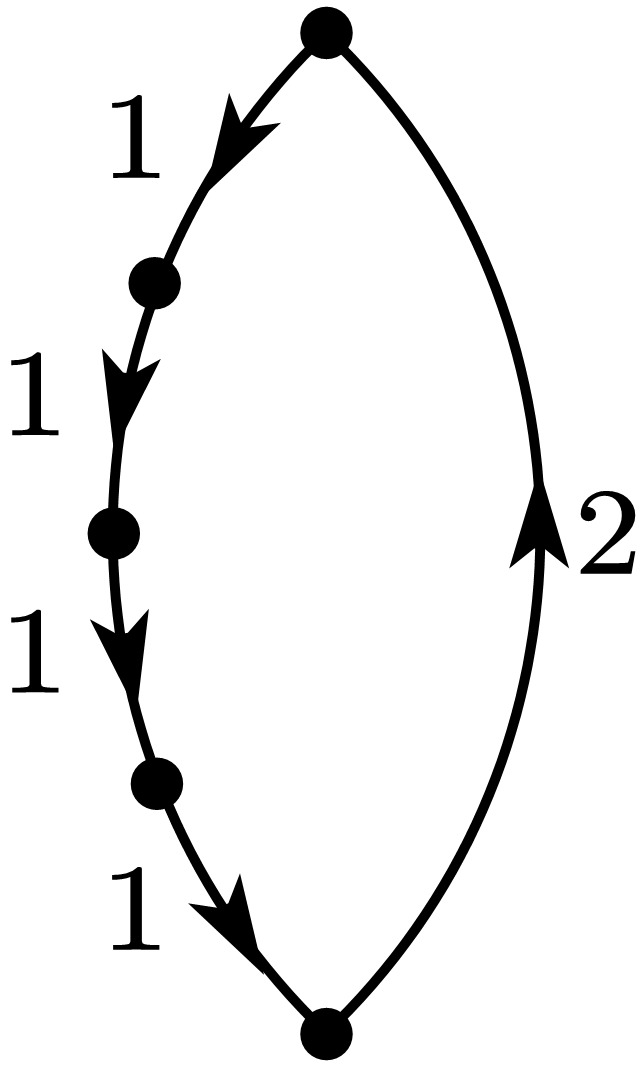
\includegraphics[scale=1.0,trim=0 -4 0 -4]{./pictures/6.01/1.png}
		\captionof*{figure}{$\displaystyle (-1)^{4+1} \frac{ V^3_{11} V_{12} V_{21} }{ ( E^{(0)}_1 - E^{(0)}_2)^4 }$}
		\end{minipage} &
		
		\begin{minipage}{0.22\linewidth}
		\centering
		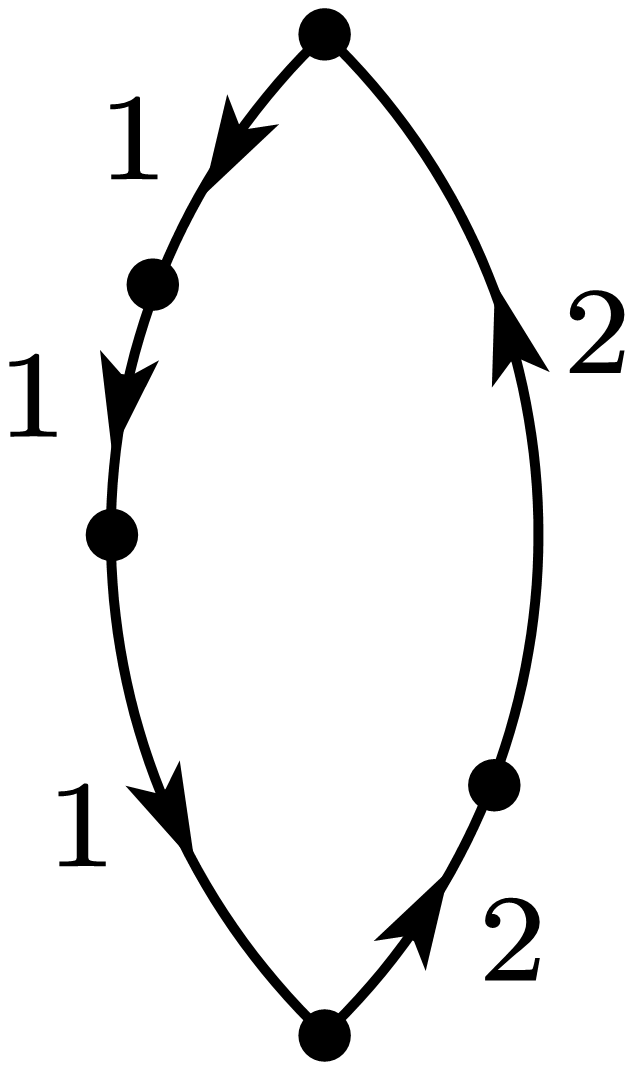
\includegraphics[scale=1.0,trim=0 -4 0 -4]{./pictures/6.01/2.png}
		\captionof*{figure}{$\displaystyle (-1)^{3+1} \frac{ V^2_{11} V_{12} V_{21} V_{22} }{ ( E^{(0)}_1 - E^{(0)}_2)^4 }$}
		\end{minipage} &
		
		\begin{minipage}{0.22\linewidth}
		\centering
		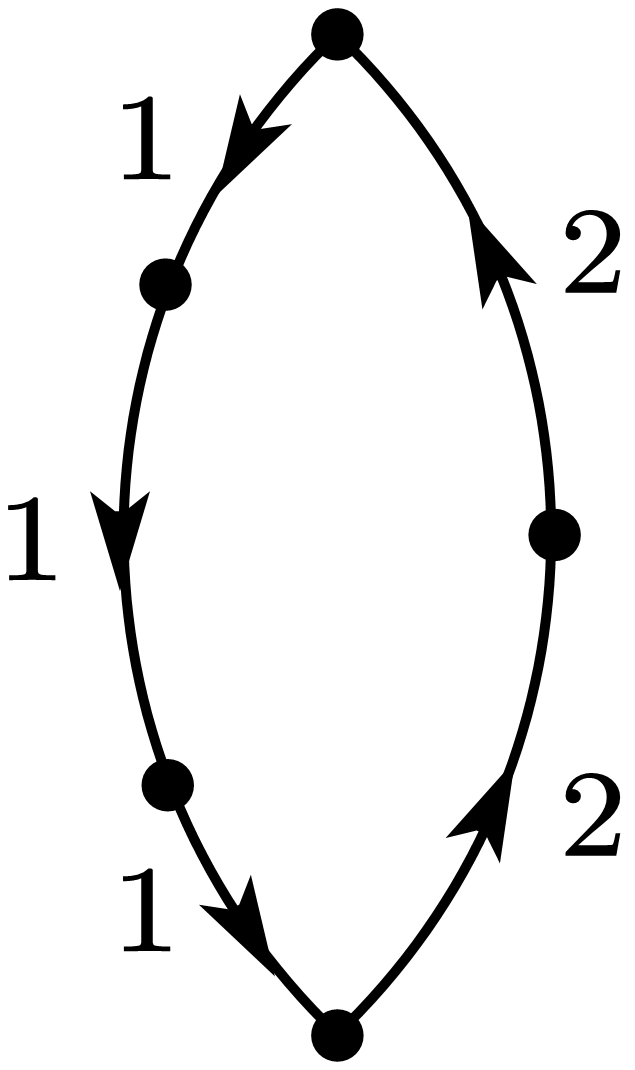
\includegraphics[scale=1.0,trim=0 -4 0 -4]{./pictures/6.01/3.png}
		\captionof*{figure}{$\displaystyle (-1)^{3+1} \frac{ V^2_{11} V_{12} V_{21} V_{22} }{ ( E^{(0)}_1 - E^{(0)}_2)^4 }$}
		\end{minipage} &
		
		\begin{minipage}{0.22\linewidth}
		\centering
		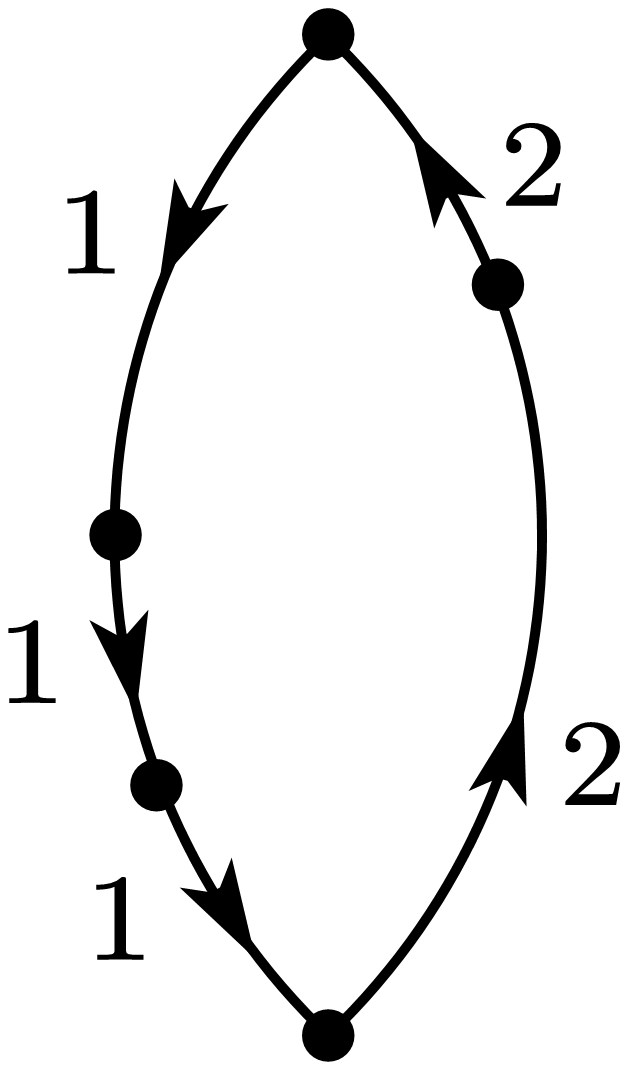
\includegraphics[scale=1.0,trim=0 -4 0 -4]{./pictures/6.01/4.png}
		\captionof*{figure}{$\displaystyle (-1)^{3+1} \frac{ V^2_{11} V_{12} V_{21} V_{22} }{ ( E^{(0)}_1 - E^{(0)}_2)^4 }$}
		\end{minipage} \\
			
		\begin{minipage}{0.22\linewidth}
		\centering
		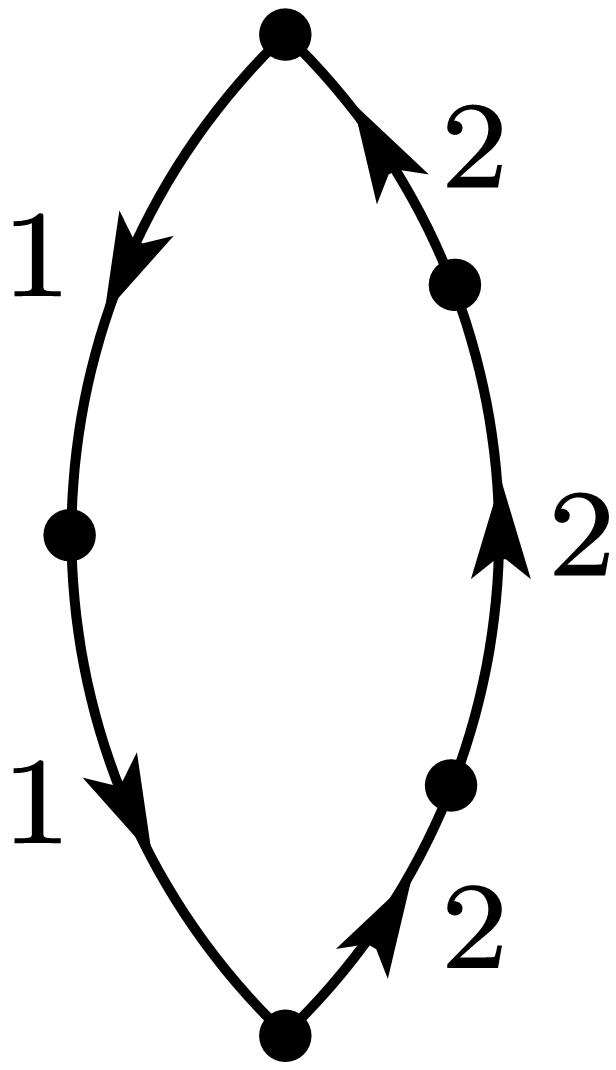
\includegraphics[scale=1.0,trim=0 -4 0 -4]{./pictures/6.01/5.png}
		\captionof*{figure}{$\displaystyle (-1)^{2+1} \frac{ V_{11} V_{12} V_{21} V^2_{22} }{ ( E^{(0)}_1 - E^{(0)}_2)^4 }$}
		\end{minipage} &
		
		\begin{minipage}{0.22\linewidth}
		\centering
		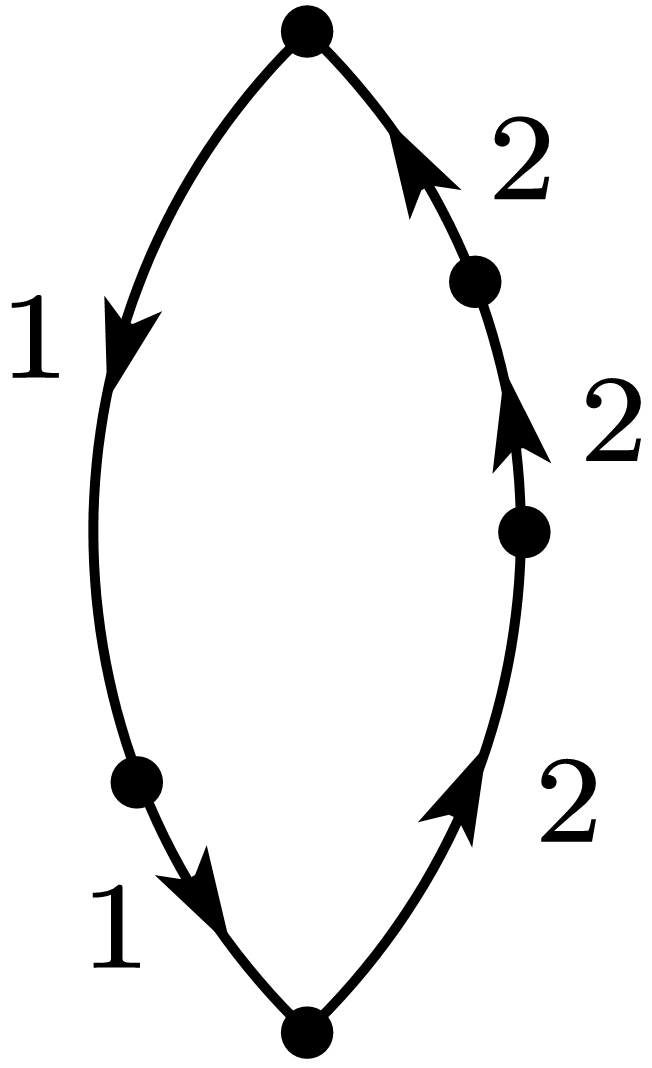
\includegraphics[scale=1.0,trim=0 -4 0 -4]{./pictures/6.01/6.png}
		\captionof*{figure}{$\displaystyle (-1)^{2+1} \frac{ V_{11} V_{12} V_{21} V^2_{22} }{ ( E^{(0)}_1 - E^{(0)}_2)^4 }$}
		\end{minipage} &
		
		\begin{minipage}{0.22\linewidth}
		\centering
		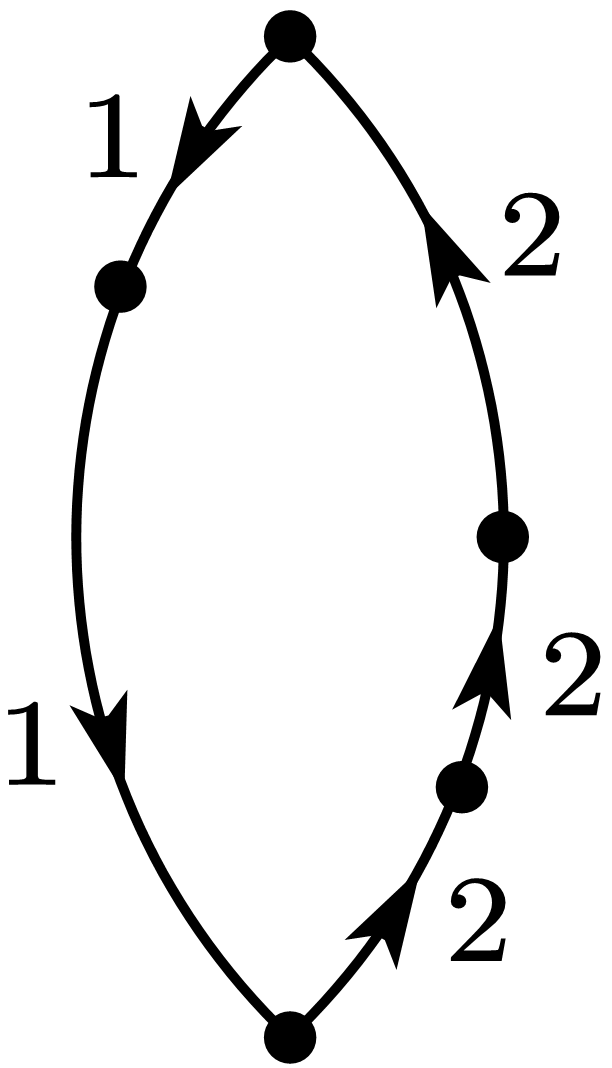
\includegraphics[scale=1.0,trim=0 -4 0 -4]{./pictures/6.01/7.png}
		\captionof*{figure}{$\displaystyle (-1)^{2+1} \frac{ V_{11} V_{12} V_{21} V^2_{22} }{ ( E^{(0)}_1 - E^{(0)}_2)^4 }$}
		\end{minipage} &
		
		\begin{minipage}{0.22\linewidth}
		\centering
		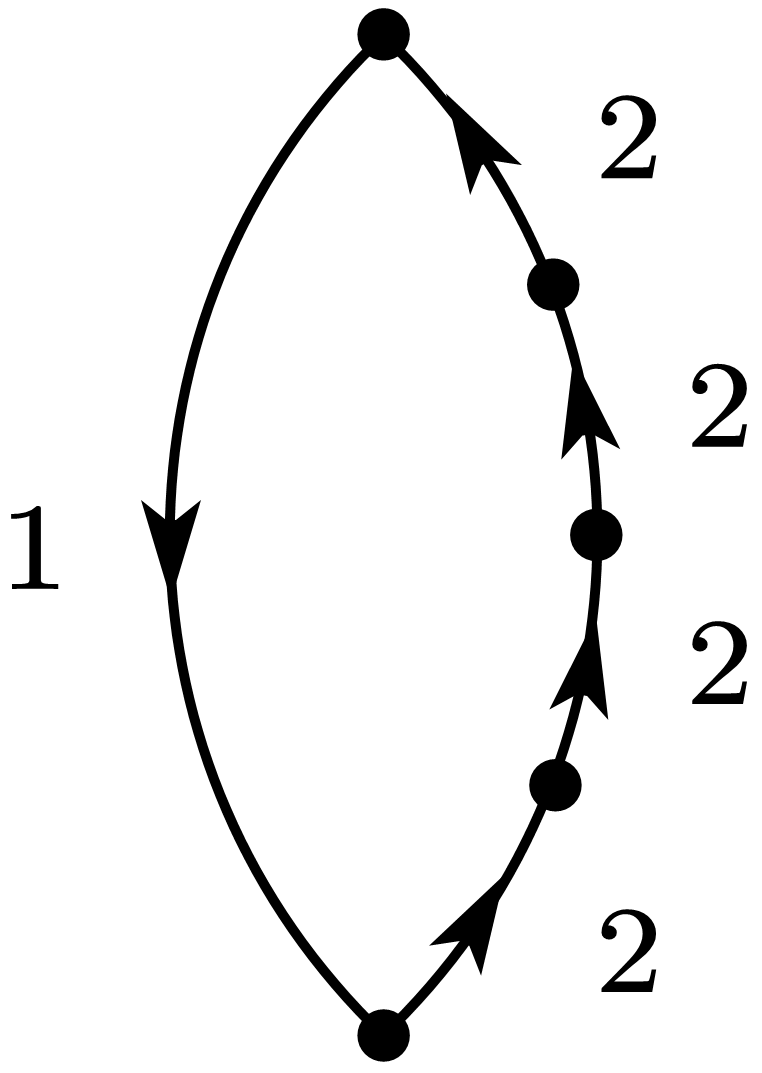
\includegraphics[scale=1.0,trim=0 -4 0 -4]{./pictures/6.01/8.png}
		\captionof*{figure}{$\displaystyle (-1)^{1+1} \frac{ V_{12} V_{21} V^3_{22} }{ ( E^{(0)}_1 - E^{(0)}_2)^4 }$}
		\end{minipage} 
		
	\end{tabular}
	\captionof{figure}{All fifth-order diagrams, which have the property that an imaginary horizontal line crosses only one hole and one particle line, and their mathematical expressions.}\label{fig:exe1}
	\end{center}
	
	Note that the diagrams, which have the property that an imaginary horizontal line crosses only one hole and one particle line, have no pair of hole/particle lines whose overlap is nonempty. For any pair of hole/particle lines which connect the dots $m_1$ and $n_1$, $m_2$ and $n_2$, where $n_1 > m_1$ and $n_2 > m_2$, their overlap will be 
	\begin{itemize}
	
	\item $[\max\{m_1, m_2\},\min\{n_1, n_2\}]$, if $\min\{n_1, n_2\} > \max\{m_1, m_2\}$;
	
	\item empty, otherwise. 
	
	\end{itemize}
	For example, if there is a pair of hole lines, one connecting the dot 1 and 3, and the other connecting 2 and 5, their overlap will be $[2, 3]$. Take an another example, if there is a pair of particle lines, one connecting the dot 5 and 4, and the other connecting 2 and 1, their overlap will be empty.
	
	Thus, there are four cases.
	\begin{itemize}
	
	\item Four hole lines and one particle line. There is only one method, hole lines are $(1,2)$, $(2,3)$, $(3,4)$, $(4,5)$ and the only particle line is $(5,1)$, as the first subdiagram in \Figref{fig:exe1}.
	
	\item Three hole lines and two particle lines. There are three methods as follows.
		\begin{itemize}
	
		\item Hole lines are $(1,2)$, $(2,3)$, and $(3,5)$ while particle lines are $(5,4)$, $(4,1)$.
		
		\item Hole lines are $(1,2)$, $(2,4)$, and $(4,5)$ while particle lines are $(5,3)$, $(3,1)$.
		
		\item Hole lines are $(1,3)$, $(3,4)$, and $(4,5)$ while particle lines are $(5,2)$, $(2,1)$.
	
		\end{itemize}
		They correspond to the second, third, fourth subdiagram in \Figref{fig:exe1}.
	
	\item Two hole lines and three particle lines. There are three methods as follows.
		\begin{itemize}
	
		\item Hole lines are $(1,3)$, $(3,5)$ while particle lines are $(5,4)$, $(4,2)$, and $(2,1)$.
		
		\item Hole lines are $(1,4)$, $(4,5)$ while particle lines are $(5,3)$, $(3,2)$, and $(2,1)$.
		
		\item Hole lines are $(1,2)$, $(2,5)$ while particle lines are $(5,4)$, $(4,3)$, and $(3,1)$.
	
		\end{itemize}
		They correspond to the fifth, sixth, seventh subdiagram in \Figref{fig:exe1}.
		
	\item One hole line and four particle lines. There is only one method, the only hole line is $(1,5)$ and particle lines are $(5,4)$, $(4,3)$, $(3,2)$, and $(2,1)$, as the eighth subdiagram in \Figref{fig:exe1}.
			
	\end{itemize}
	
	Thus, the sum of such diagrams is
	\begin{align*}
%		&\hspace{1.4em}(-1)^{4+1} \frac{ V^3_{11} V_{12} V_{21} }{ ( E^{(0)}_1 - E^{(0)}_2)^4 } + (-1)^{3+1} \frac{ V^2_{11} V_{12} V_{21} V_{22} }{ ( E^{(0)}_1 - E^{(0)}_2)^4 } + (-1)^{3+1} \frac{ V^2_{11} V_{12} V_{21} V_{22} }{ ( E^{(0)}_1 - E^{(0)}_2)^4 } \\
%		&\hspace{1.4em} + (-1)^{3+1} \frac{ V^2_{11} V_{12} V_{21} V_{22} }{ ( E^{(0)}_1 - E^{(0)}_2)^4 } + (-1)^{2+1} \frac{ V_{11} V_{12} V_{21} V^2_{22} }{ ( E^{(0)}_1 - E^{(0)}_2) }^4 + (-1)^{2+1} \frac{ V_{11} V_{12} V_{21} V^2_{22} }{ ( E^{(0)}_1 - E^{(0)}_2) }^4 \\
%		&\hspace{1.4em}  + (-1)^{2+1} \frac{ V_{11} V_{12} V_{21} V^2_{22} }{ ( E^{(0)}_1 - E^{(0)}_2) }^4 + (-1)^{1+1} \frac{ V_{12} V_{21} V^3_{22} }{ ( E^{(0)}_1 - E^{(0)}_2)^4 } \\
%		&= - \frac{ V^3_{11} V_{12} V_{21} }{ ( E^{(0)}_1 - E^{(0)}_2)^4 } + 3 \frac{ V^2_{11} V_{12} V_{21} V_{22} }{ ( E^{(0)}_1 - E^{(0)}_2)^4 } - 3 \frac{ V_{11} V_{12} V_{21} V^2_{22} }{ ( E^{(0)}_1 - E^{(0)}_2) }^4 + \frac{ V_{12} V_{21} V^3_{22} }{ ( E^{(0)}_1 - E^{(0)}_2)^4 } \\
%		&= 
		- \frac{ V_{12} V_{21} \left( V^3_{11} - 3 V^2_{11} V_{22} + 3 V_{11} V_{22} - V^3_{22} \right) }{ ( E^{(0)}_1 - E^{(0)}_2)^4 } = - \frac{ V_{12} V_{21} \left( V_{11} - V_{22} \right)^3 }{ ( E^{(0)}_1 - E^{(0)}_2)^4 } = \frac{ V_{12} V_{21} \left( V_{22} - V_{11} \right)^3 }{ ( E^{(0)}_1 - E^{(0)}_2)^4 }.
	\end{align*}
	
	In fact, as the textbook says, these eight diagrams can be generated by adding three dots to the second-order diagram in all positive ways. In fact, any pair of hole/particle lines in them has also empty overlap. I think the calculation of the overlap is much direct than inspecting the property of lines.
	
	\end{solution}

	\subsection{Diagrammatic Perturbation Theory for \texorpdfstring{$N$}- States}
	
	% 6.2
	\begin{exercise}
	Use diagrammatic techniques to obtain the fourth-order perturbation energy of a particular state (say, $i$) of an $N$-state system. That is, evaluate the diagrams
	
	\begin{center}
	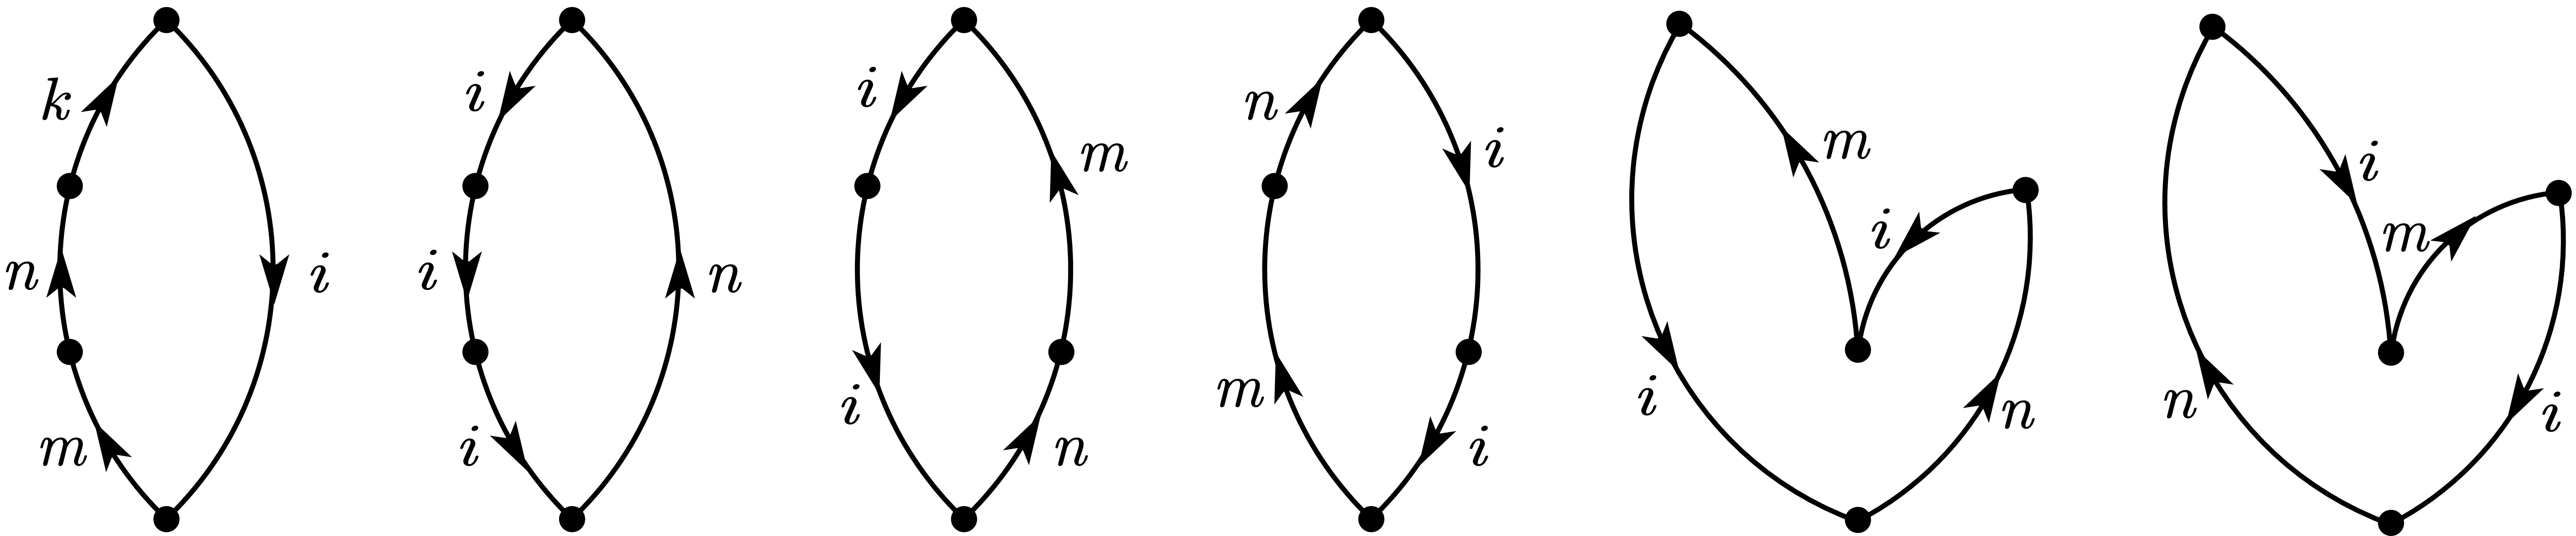
\includegraphics[scale=1.0]{./pictures/6.02/exercise.png}
	\end{center}
	
	where the indices $m$, $n$, $k$, ... exclude $i$. Using the approach of Section 6.1, obtain an algebraic expression for the fourth-order energy and compare it to the diagrammatic result.
	
	\end{exercise}
	
	\begin{solution}
	
	\begin{center}
	\begin{tabular}{cc}
	
		\begin{minipage}{0.49\linewidth}
		\centering
		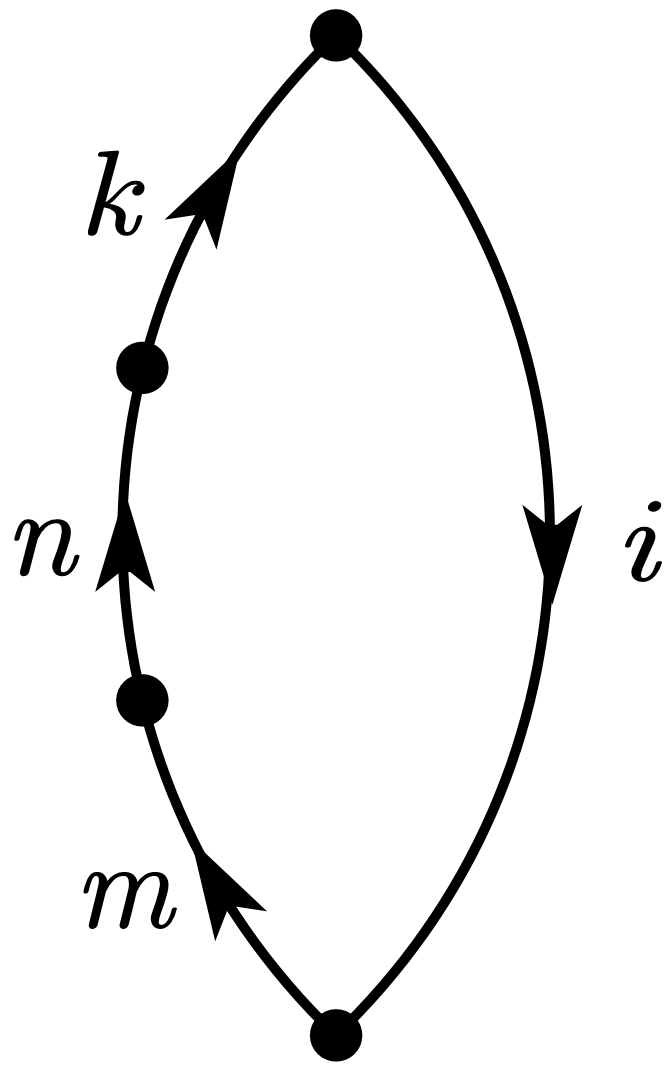
\includegraphics[scale=1.0,trim=0 -4 0 -4]{./pictures/6.02/1.png}
		\captionof*{figure}{$(-1)^{1+1} { \sum_{kmn} }^\prime \frac{ V_{ki} V_{nk} V_{mn} V_{im} }{ ( E^{(0)}_i - E^{(0)}_k ) ( E^{(0)}_i - E^{(0)}_n ) ( E^{(0)}_i - E^{(0)}_m ) }$}
		\end{minipage} &
		
		\begin{minipage}{0.42\linewidth}
		\centering
		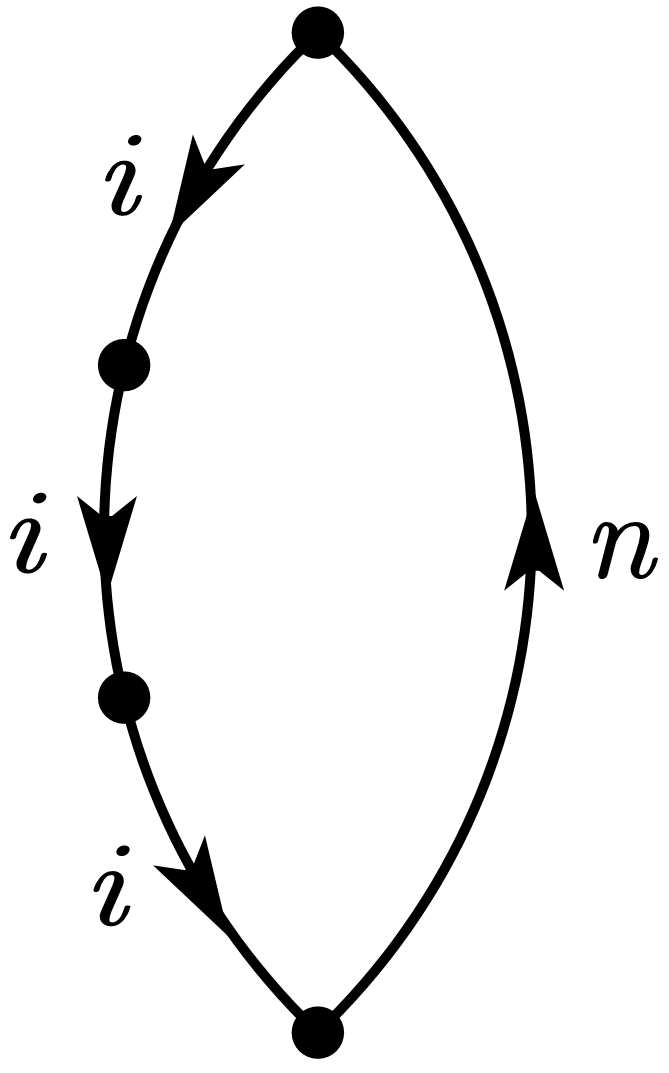
\includegraphics[scale=1.0,trim=0 -4 0 -4]{./pictures/6.02/2.png}
		\captionof*{figure}{$(-1)^{3+1} { \sum_n }^\prime \frac{ V_{ni} V^2_{ii} V_{in} }{ ( E^{(0)}_i - E^{(0)}_n)^3 }$}
		\end{minipage} \\
		
		\begin{minipage}{0.49\linewidth}
		\centering
		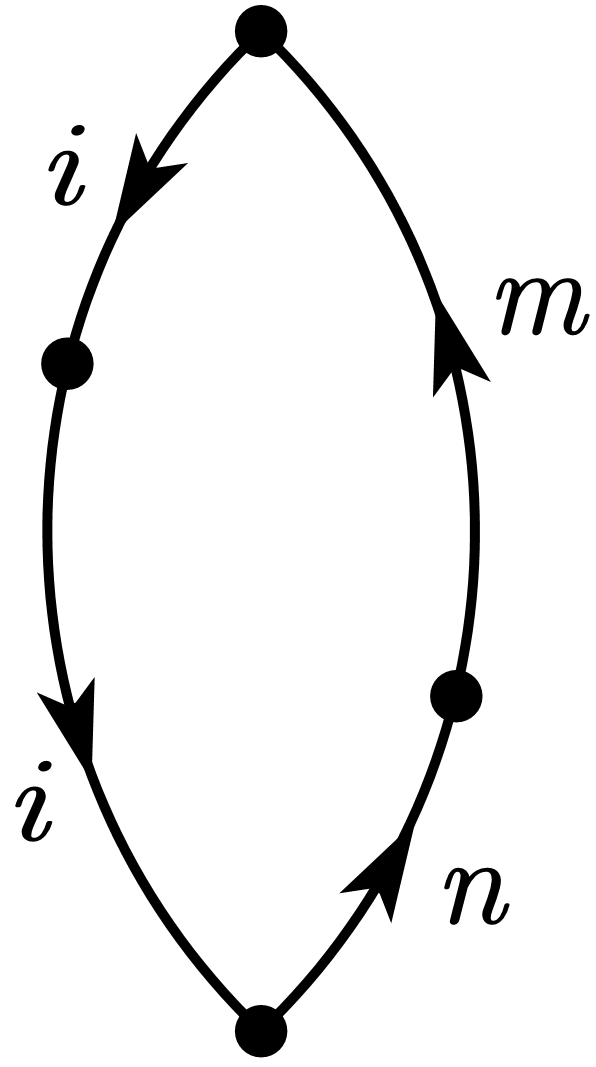
\includegraphics[scale=1.0,trim=0 -4 0 -4]{./pictures/6.02/3.png}
		\captionof*{figure}{$(-1)^{2+1} { \sum_{mn} }^\prime \frac{ V_{mi} V_{ii} V_{in} V_{nm} }{ ( E^{(0)}_i - E^{(0)}_n) ( E^{(0)}_i - E^{(0)}_m )^2 }$}
		\end{minipage}  &
			
		\begin{minipage}{0.42\linewidth}
		\centering
		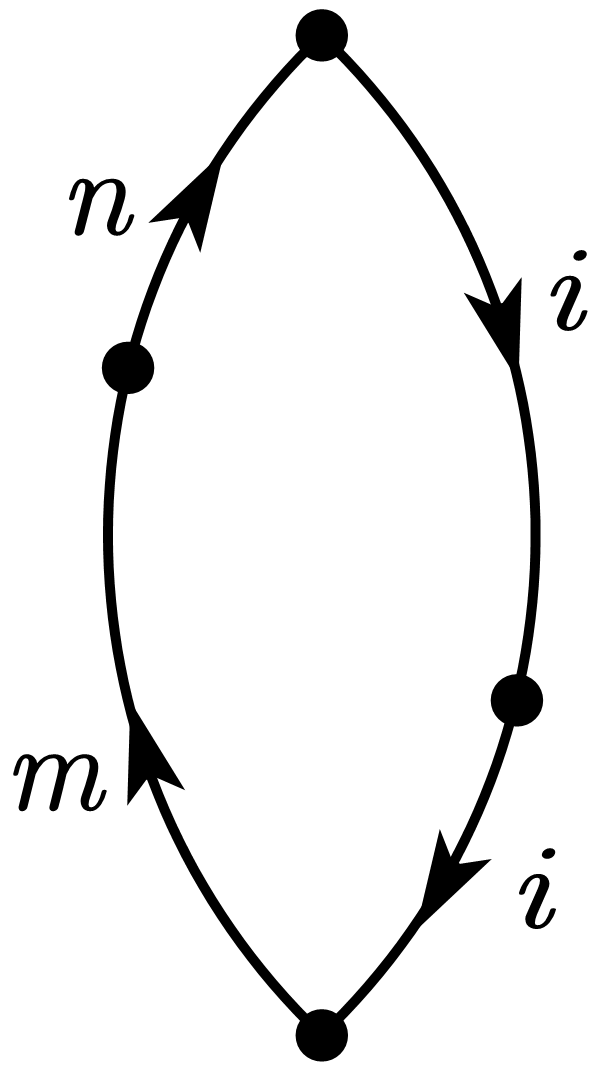
\includegraphics[scale=1.0,trim=0 -4 0 -4]{./pictures/6.02/4.png}
		\captionof*{figure}{$(-1)^{2+1} { \sum_{mn} }^\prime \frac{ V_{ni} V_{ii} V_{im} V_{mn} }{ ( E^{(0)}_i - E^{(0)}_n) ( E^{(0)}_i - E^{(0)}_m )^2 }$}
		\end{minipage} \\
		
		\begin{minipage}{0.49\linewidth}
		\centering
		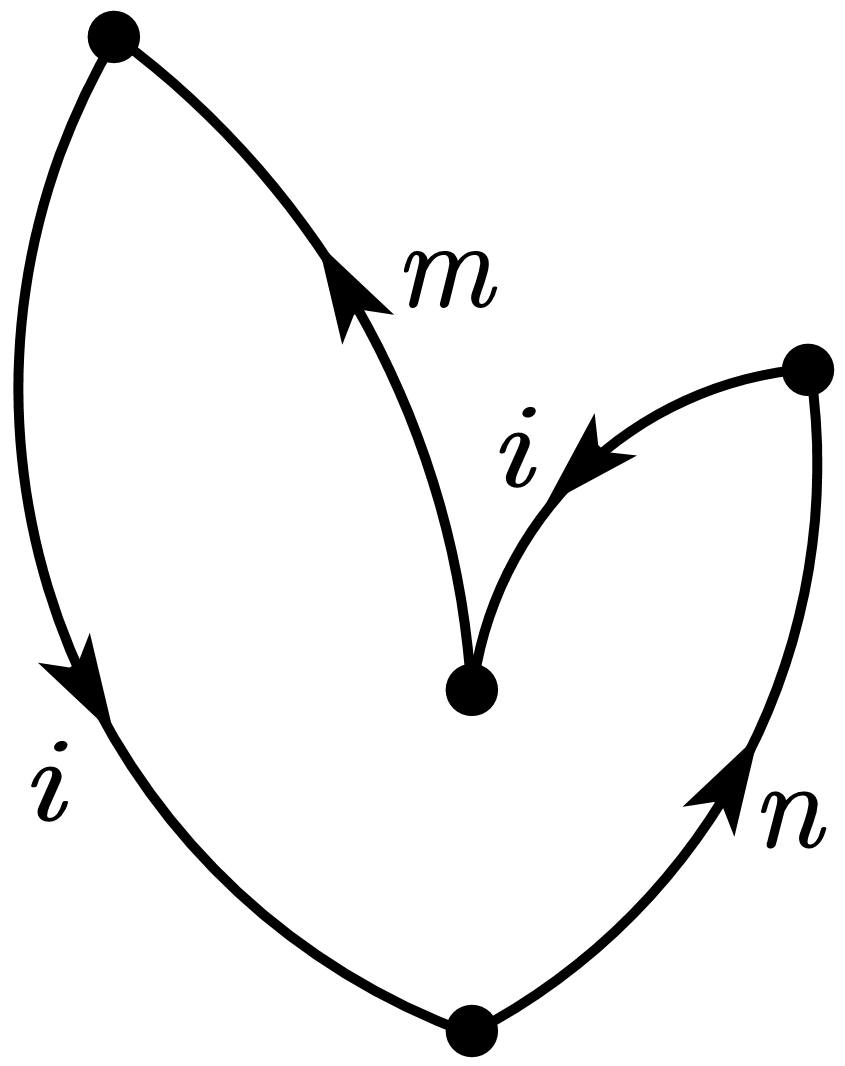
\includegraphics[scale=1.0,trim=0 -4 0 -4]{./pictures/6.02/5.png}
		\captionof*{figure}{$(-1)^{2+1} { \sum_{mn} }^\prime \frac{ V_{mi} V_{in} V_{ni} V_{im} }{ ( E^{(0)}_i - E^{(0)}_m ) ( 2E^{(0)}_i - E^{(0)}_m - E^{(0)}_n ) ( E^{(0)}_i - E^{(0)}_n ) }$}
		\end{minipage} &
		
		\begin{minipage}{0.42\linewidth}
		\centering
		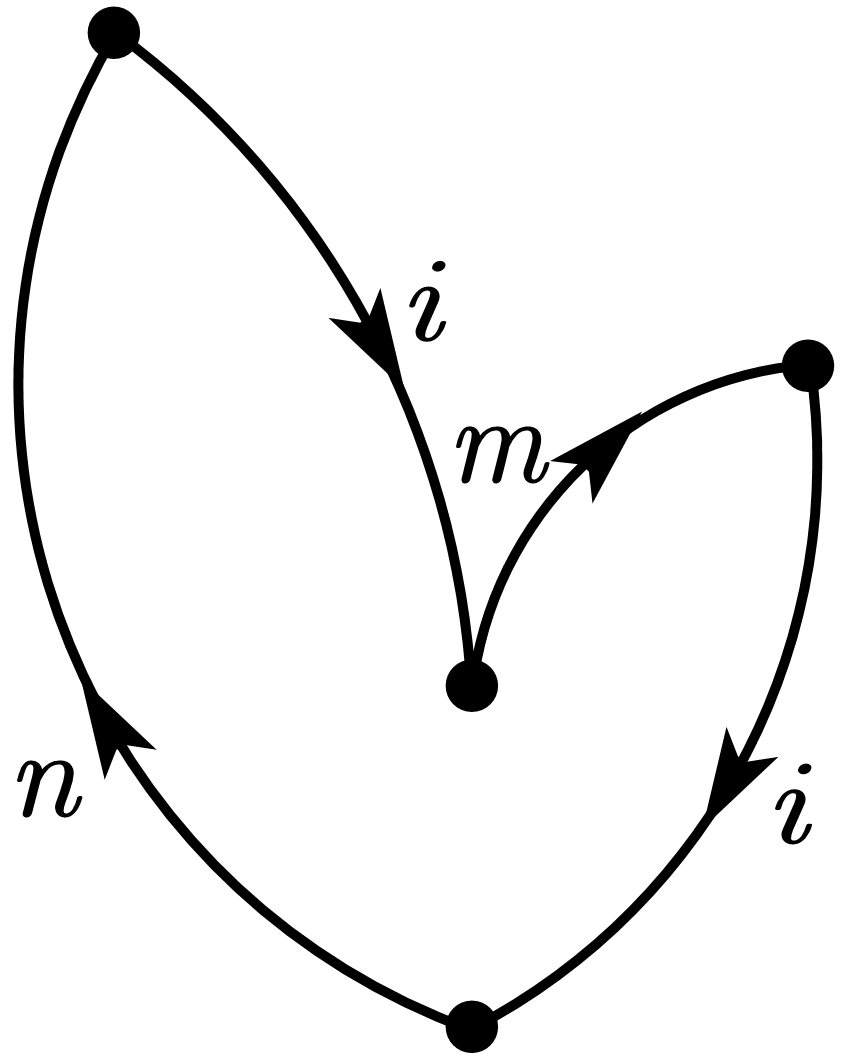
\includegraphics[scale=1.0,trim=0 -4 0 -4]{./pictures/6.02/6.png}
		\captionof*{figure}{$(-1)^{2+1} { \sum_{mn} }^\prime \frac{ V_{in} V_{ni} V_{im} V_{mi} }{ ( 2E^{(0)}_i - E^{(0)}_m - E^{(0)}_n ) ( E^{(0)}_i - E^{(0)}_n )^2 }$}
		\end{minipage} 
				
	\end{tabular}
	\captionof{figure}{All fourth-order diagrams and their mathematical expressions.}\label{fig:exe2}
	\end{center}
	
%	\begin{align*}
%		E^{(4)}_i &= (-1)^{1+1} { \sum_{kmn} }^\prime \frac{ V_{ki} V_{nk} V_{mn} V_{im} }{ ( E^{(0)}_i - E^{(0)}_k ) ( E^{(0)}_i - E^{(0)}_n ) ( E^{(0)}_i - E^{(0)}_m ) } + (-1)^{3+1} { \sum_n }^\prime \frac{ V_{ni} V^2_{ii} V_{in} }{ ( E^{(0)}_i - E^{(0)}_n)^3 } \\
%		&\hspace{2em} + (-1)^{2+1} { \sum_{mn} }^\prime \frac{ V_{mi} V_{ii} V_{in} V_{nm} }{ ( E^{(0)}_i - E^{(0)}_n) ( E^{(0)}_i - E^{(0)}_m )^2 } + (-1)^{2+1} { \sum_{mn} }^\prime \frac{ V_{ni} V_{ii} V_{im} V_{mn} }{ ( E^{(0)}_i - E^{(0)}_n) ( E^{(0)}_i - E^{(0)}_m )^2 } \\
%		&\hspace{2em} + (-1)^{2+1} { \sum_{mn} }^\prime \frac{ V_{mi} V_{in} V_{ni} V_{im} }{ ( E^{(0)}_i - E^{(0)}_m ) ( 2E^{(0)}_i - E^{(0)}_m - E^{(0)}_n ) ( E^{(0)}_i - E^{(0)}_n ) } \\
%		&\hspace{2em} + (-1)^{2+1} { \sum_{mn} }^\prime \frac{ V_{in} V_{ni} V_{im} V_{mi} }{ ( 2E^{(0)}_i - E^{(0)}_m - E^{(0)}_n ) ( E^{(0)}_i - E^{(0)}_n )^2 } \\
%	\end{align*}

htrETWREARHSTJ
	
	\begin{align*}
		E^{(4)}_i &= \langle i | \mathscr{V} | \Psi^{(3)}_i \rangle = { \sum_n }^\prime \langle i | \mathscr{V} | n \rangle \langle n | \Psi^{(3)}_i \rangle \\
		&= { \sum_n }^\prime \frac{ V_{in} }{ E^{(0)}_i - E^{(0)}_n } \left[ \langle n | \mathscr{V} | \Psi^{(2)}_i \rangle - E^{(1)}_i \langle n | \Psi^{(2)}_i \rangle - E^{(2)}_i \langle n | \Psi^{(1)}_i \rangle \right] \\
		&= { \sum_n }^\prime \frac{ V_{in} \langle n | \mathscr{V} | \Psi^{(2)}_i \rangle }{ E^{(0)}_i - E^{(0)}_n } - E^{(1)}_i { \sum_n }^\prime \frac{ V_{in} \langle n | \Psi^{(2)}_i \rangle }{ E^{(0)}_i - E^{(0)}_n } - E^{(2)}_i { \sum_n }^\prime \frac{ V_{in} \langle n | \mathscr{V} | \Psi^{(1)}_i \rangle }{ E^{(0)}_i - E^{(0)}_n } \\
		&= { \sum_{mn} }^\prime \frac{ V_{in} \langle n | \mathscr{V} | m \rangle \langle m | \Psi^{(2)}_i \rangle }{ E^{(0)}_i - E^{(0)}_n } - E^{(1)}_i { \sum_n }^\prime \frac{ V_{in} }{ E^{(0)}_i - E^{(0)}_n } \langle n | \Psi^{(2)}_i \rangle - E^{(2)}_i { \sum_{mn} }^\prime \frac{ V_{in} \langle n | \mathscr{V} | m \rangle \langle m | \Psi^{(1)}_i \rangle }{ E^{(0)}_i - E^{(0)}_n } \\
		&= { \sum_{mn} }^\prime \frac{ V_{in} V_{nm} }{ E^{(0)}_i - E^{(0)}_n } \langle m | \Psi^{(2)}_i \rangle - { \sum_n }^\prime \frac{ V_{ii} V_{in} }{ E^{(0)}_i - E^{(0)}_n } \langle n | \Psi^{(2)}_i \rangle - \left( { \sum_k }^\prime \frac{ V_{ik} V_{ki} }{ E^{(0)}_i - E^{(0)}_k } \right) { \sum_{mn} }^\prime \frac{ V_{in} V_{nm} \langle m | \Psi^{(1)}_i \rangle }{ E^{(0)}_i - E^{(0)}_n } \\
		&= { \sum_{mn} }^\prime \frac{ V_{in} V_{nm} }{ E^{(0)}_i - E^{(0)}_n } \frac{ \langle m | \mathscr{V} | \Psi^{(1)}_i \rangle - E^{(1)}_i \langle m | \Psi^{(1)}_i \rangle }{ E^{(0)}_i - E^{(0)}_m } - { \sum_n }^\prime \frac{ V_{ii} V_{in} }{ E^{(0)}_i - E^{(0)}_n } \frac{ \langle n | \mathscr{V} | \Psi^{(1)}_i \rangle - E^{(1)}_i \langle n | \Psi^{(1)}_i \rangle }{ E^{(0)}_i - E^{(0)}_n } \\
		&\hspace{2em} - \left( { \sum_k }^\prime \frac{ V_{ik} V_{ki} }{ E^{(0)}_i - E^{(0)}_k } \right) { \sum_{mn} }^\prime \frac{ V_{in} V_{nm} }{ E^{(0)}_i - E^{(0)}_n } \langle m | \Psi^{(1)}_i \rangle \\
		&= { \sum_{mn} }^\prime \frac{ V_{in} V_{nm} }{ (E^{(0)}_i - E^{(0)}_n) (E^{(0)}_i - E^{(0)}_m) } \left[ { \sum_k }^\prime \langle m | \mathscr{V} | k \rangle \langle k | \Psi^{(1)}_i \rangle - E^{(1)}_i \langle m | \Psi^{(1)}_i \rangle \right] \\
		&\hspace{2em} - { \sum_n }^\prime \frac{ V_{ii} V_{in} }{ ( E^{(0)}_i - E^{(0)}_n )^2 } \left[ { \sum_m }^\prime \langle n | \mathscr{V} | m \rangle \langle m | \Psi^{(1)}_i \rangle - E^{(1)}_i \langle n | \Psi^{(1)}_i \rangle \right] - { \sum_{mnk} }^\prime \frac{ V_{ik} V_{ki} V_{in} V_{nm} \langle m | \Psi^{(1)}_i \rangle }{ ( E^{(0)}_i - E^{(0)}_n ) ( E^{(0)}_i - E^{(0)}_k ) }  \\
		&= { \sum_{mnk} }^\prime \frac{ V_{in} V_{nm} V_{mk} }{ (E^{(0)}_i - E^{(0)}_n) (E^{(0)}_i - E^{(0)}_m) } \langle k | \Psi^{(1)}_i \rangle - { \sum_{mn} }^\prime \frac{ V_{ii} V_{in} V_{nm} }{ (E^{(0)}_i - E^{(0)}_n) (E^{(0)}_i - E^{(0)}_m) } \langle m | \Psi^{(1)}_i \rangle \\
		&\hspace{2em} - { \sum_{mn} }^\prime \frac{ V_{ii} V_{in} V_{nm} }{ ( E^{(0)}_i - E^{(0)}_n )^2 } \langle m | \Psi^{(1)}_i \rangle + { \sum_n }^\prime \frac{ V^2_{ii} V_{in} }{ ( E^{(0)}_i - E^{(0)}_n )^2 } \langle n | \Psi^{(1)}_i \rangle - { \sum_{mnk} }^\prime \frac{ V_{ik} V_{ki} V_{in} V_{nm} \langle m | \Psi^{(1)}_i \rangle }{ ( E^{(0)}_i - E^{(0)}_n ) ( E^{(0)}_i - E^{(0)}_k ) } \\ 
	\end{align*}
	
	\end{solution}
	
	\subsection{Summation of Diagrams}
	
	\section{Orbital Perturbation Theory: One-Particle Perturbations}	

\end{document}
